\documentclass[12pt,a4paper]{article}

% ── Codificación y lengua ──
\usepackage[utf8]{inputenc}
\usepackage[T1]{fontenc}
\usepackage{babel}
\babelprovide[main, import]{spanish}

% ── Layout ──
\usepackage[margin=2.5cm]{geometry}
\usepackage{parskip}

% ── Tipografía ──
\usepackage{lmodern}

% ── Figuras, tablas, código ──
\usepackage{graphicx}
\usepackage{booktabs}
\usepackage{tabularx}
\usepackage{float}
\usepackage[table]{xcolor}
\usepackage{listings}
\usepackage{amsmath,amssymb}
\usepackage{hyperref}
\usepackage{caption}

% ── Configuración de listings ──
\definecolor{codebg}{HTML}{F5F5F5}
\definecolor{codeframe}{HTML}{CCCCCC}
\definecolor{kw}{HTML}{0000CC}
\definecolor{str}{HTML}{008800}
\definecolor{cmt}{HTML}{888888}

\lstset{
  backgroundcolor=\color{codebg},
  frame=single,
  rulecolor=\color{codeframe},
  basicstyle=\ttfamily\small,
  keywordstyle=\color{kw}\bfseries,
  stringstyle=\color{str},
  commentstyle=\color{cmt}\itshape,
  breaklines=true,
  numbers=left,
  numberstyle=\tiny\color{cmt},
  numbersep=8pt,
  tabsize=4,
  showstringspaces=false,
  captionpos=b
}

\hypersetup{colorlinks=true, linkcolor=blue!60!black, urlcolor=blue!60!black, citecolor=blue!60!black}

% ── Ruta de imágenes ──
\graphicspath{{img/}}

% ══════════════════════════════════════════════════════════════════
\begin{document}

\begin{titlepage}
\centering
\vspace*{3cm}
{\LARGE\bfseries Resiliencia de la Internet chilena\\ante un terremoto M8.8\par}
\vspace{1.5cm}
{\Large Tarea 2 Individual --- Ruteo\par}
\vspace{2cm}
{\large
Curso: Ruteo en Redes de Telecomunicaciones\\[6pt]
Noviembre 2026\par}
\vfill
{\small Basado en el estudio CORFO 15BPE-47225\\
(U.\ de Chile / NIC Labs, 2018)\par}
\end{titlepage}

\tableofcontents
\newpage

% ══════════════════════════════════════════════════════════════════
\section{Introducción}

La infraestructura de telecomunicaciones constituye un sistema crítico cuya
continuidad operativa resulta esencial durante y después de un desastre
natural.  Chile, por su ubicación en el denominado \emph{Cinturón de Fuego
del Pacífico}, está expuesto a sismos de gran magnitud que pueden afectar
simultáneamente grandes extensiones de la red de fibra óptica.  El presente
informe analiza la resiliencia de dicha red frente a un escenario sísmico
concreto: el terremoto M8.8 del Maule, ocurrido el 27 de febrero de 2010.

Para ello se construye un modelo computacional sobre \textbf{PostgreSQL +
PostGIS + pgRouting} que integra datos geográficos oficiales de la red,
identifica los nodos clave del país, calcula la métrica \textbf{ATTR}
(All-Terminal Reliability) antes y después del sismo mediante simulación
\textbf{Monte Carlo}, y visualiza los resultados en un mapa interactivo
\textbf{Leaflet}.

El flujo completo se ejecuta con un solo orquestador:

\begin{lstlisting}[language=bash,caption={Ejecución del proyecto}]
python main.py all           # initdb + attr + serve
\end{lstlisting}


% ══════════════════════════════════════════════════════════════════
\section{Datos y fuente}

La infraestructura analizada proviene del proyecto \textbf{Yafún} (NIC
Chile) y del estudio \emph{``Estudio y Recomendaciones sobre la Resiliencia
de la infraestructura de la Internet chilena''}, Informe Técnico Final
CORFO 15BPE-47225 (U.\ de Chile / NIC Labs, diciembre 2018)~\cite{niclabs2018}.  Los datos geográficos fueron entregados por SUBTEL vía
solicitud de transparencia como \textit{shapefiles} en WGS84 (EPSG:4326) y
comprenden cuatro capas que se resumen en la Tabla~\ref{tab:capas}.

\begin{table}[H]
\centering
\caption{Capas de infraestructura cargadas}
\label{tab:capas}
\begin{tabular}{lrrp{5cm}}
\toprule
\textbf{Capa} & \textbf{Tramos} & \textbf{Largo (km)} & \textbf{Uso en el modelo} \\
\midrule
\texttt{fibra\_optica\_detectada}     & 1.915 & 10.313 & Arista operativa \\
\texttt{trayecto\_en\_ferry}          &   204 &  2.390 & Arista operativa \\
\texttt{postacion\_electrica\_detectada} & 1.213 & 6.712 & Potencial \\
\texttt{camino\_sin\_postacion\_detectado} & 1.165 & 8.108 & Potencial \\
\midrule
\multicolumn{2}{l}{\textbf{Total}} & $\approx$27.500 & \\
\bottomrule
\end{tabular}
\end{table}

El total es consistente con los ``28.000 km'' reportados por el proyecto.
La red \textbf{en operación} se define como la unión de las capas de fibra
óptica y trayecto en ferry, ya que son las únicas que transportan datos
efectivamente.  Las capas de postación eléctrica y caminos sin postación
representan infraestructura \textit{potencial} ---~lugares donde se podría
tender fibra a menor costo, como las emplea el estudio en su modelo de
optimización~--- pero no cursan tráfico.

La carga de los \textit{shapefiles} en la base de datos se realiza mediante
\texttt{shp2pgsql}, invocado desde el orquestador \texttt{main.py}:

\begin{lstlisting}[language=Python,caption={Carga de shapefiles (main.py)}]
LAYERS = [
    "fibra_optica_detectada",
    "postacion_electrica_detectada",
    "camino_sin_postacion_detectado",
    "trayecto_en_ferry",
]

for lyr in LAYERS:
    shp = os.path.join(SHPDIR, lyr + ".shp")
    sqlgen = subprocess.run(
        ["shp2pgsql", "-I", "-s", "4326", "-d", shp, lyr],
        capture_output=True, text=True, check=True)
    subprocess.run(
        ["psql", *_psql_args(DSN), "-q",
         "-v", "ON_ERROR_STOP=1"],
        input=sqlgen.stdout, text=True)
\end{lstlisting}


% ══════════════════════════════════════════════════════════════════
\section{Nodos clave}

Para evaluar la resiliencia de la red es necesario definir cuáles son los
puntos que generan, intercambian y reciben información.  Siguiendo el
criterio del estudio de referencia~\cite{niclabs2018}, se seleccionaron
\textbf{19 ciudades} que cumplen roles diferenciados en la topología de
la Internet nacional.

En primer lugar se encuentran los nodos de \textbf{intercambio}: Santiago
---~sede del PIT Chile / NAP y mayor concentración de \textit{data
centers}~--- junto con los hubs regionales de Valparaíso, Antofagasta, La
Serena, Concepción, Temuco, Puerto Montt y Punta Arenas.  En segundo lugar
se consideran los nodos de \textbf{generación y recepción}: las capitales
regionales y ciudades cabecera que agregan y distribuyen el tráfico de su
zona, incluyendo Arica, Iquique, Calama, Copiapó, Rancagua, Talca,
Chillán, Valdivia, Osorno, Castro y Coyhaique.

Para vincular cada ciudad con la topología de la red, cada nodo clave se
\textit{engancha} al vértice más cercano de la red en operación mediante
\texttt{ST\_Distance} sobre geografía:

\begin{lstlisting}[language=SQL,caption={Snap de nodos clave a la red (03\_nodos\_clave.sql)}]
WITH snap AS (
    SELECT n.cod,
           v.id AS vid,
           ST_Distance(n.geom::geography,
                       v.the_geom::geography) AS d
    FROM nodos_clave n
    CROSS JOIN LATERAL (
        SELECT ev.id, ev.the_geom
        FROM edges_vertices_pgr ev
        WHERE EXISTS (
            SELECT 1 FROM edges e
            WHERE e.operativo
              AND (e.source=ev.id OR e.target=ev.id))
        ORDER BY n.geom <-> ev.the_geom
        LIMIT 1
    ) v
)
UPDATE nodos_clave n
SET vertex_id = snap.vid,
    dist_m    = snap.d
FROM snap WHERE snap.cod = n.cod;
\end{lstlisting}


% ══════════════════════════════════════════════════════════════════
\section{Topología de red y \texttt{pgr\_createTopology}}

La construcción de la topología parte por unificar las cuatro capas de
infraestructura en una sola tabla \texttt{edges}.  Dado que algunas
geometrías son \texttt{MultiLineString}, se descomponen en segmentos
simples mediante \texttt{ST\_Dump}, asignando a cada arista un costo
bidireccional igual a su largo en metros:

\begin{lstlisting}[language=SQL,caption={Tabla unificada de aristas (02\_topologia.sql)}]
INSERT INTO edges (tipo, operativo, src_id, geom, cost, reverse_cost)
SELECT 'fibra', true, id::text, (ST_Dump(geom)).geom,
       ST_Length((ST_Dump(geom)).geom::geography),
       ST_Length((ST_Dump(geom)).geom::geography)
FROM fibra_optica_detectada;
-- (idem para ferry, postacion, camino)
\end{lstlisting}

\subsection{Compatibilidad con pgRouting 4.x}

Un aspecto técnico relevante es que pgRouting \textbf{4.0} eliminó la
función \texttt{pgr\_createTopology}, reemplazándola por
\texttt{pgr\_extractVertices}.  Sin embargo, como el enunciado de la tarea
exige explícitamente el uso de \texttt{pgr\_createTopology}, se implementó
una \textbf{función de compatibilidad} que reproduce la misma firma y
comportamiento de la función original.  Internamente utiliza
\texttt{ST\_ClusterDBSCAN} con \texttt{eps = tolerancia} para agrupar los
extremos cercanos de las aristas en un mismo vértice lógico, genera la
tabla \texttt{edges\_vertices\_pgr} con el centroide de cada cluster, y
rellena las columnas \texttt{source}/\texttt{target}:

\begin{lstlisting}[language=SQL,caption={Función de compatibilidad pgr\_createTopology (fragmento)}]
CREATE OR REPLACE FUNCTION pgr_createTopology(
    edge_table  text,
    tolerance   double precision,
    the_geom    text DEFAULT 'geom',
    id          text DEFAULT 'id',
    source      text DEFAULT 'source',
    target      text DEFAULT 'target',
    rows_where  text DEFAULT 'true',
    clean       boolean DEFAULT false
) RETURNS text LANGUAGE plpgsql AS $$
DECLARE
    vtable text := edge_table || '_vertices_pgr';
BEGIN
    -- 1. Reunir extremos de las aristas (inicio y fin)
    -- 2. Clustering con ST_ClusterDBSCAN(pt, eps:=tolerance)
    -- 3. Generar tabla de vertices (centroide de cada cluster)
    -- 4. Rellenar source/target de cada arista
    ...
END; $$;
\end{lstlisting}

La invocación es idéntica a la función original:

\begin{lstlisting}[language=SQL,caption={Invocación de pgr\_createTopology}]
SELECT pgr_createTopology('edges', 0.005, 'geom', 'id');
\end{lstlisting}

\subsection{Resultado de la topología}

La tolerancia seleccionada fue de 0.005° (aproximadamente 555~m),
calibrada mediante pruebas en el rango 0.001--0.02; con este valor se
cierran los huecos de digitalización sin fusionar nodos que realmente son
distintos.  El resultado es un grafo de \textbf{4.268 vértices} y
\textbf{4.497 aristas}, con un grado medio de 2.06 y un máximo de~7.

Un hallazgo fundamental es la \textbf{fragmentación} de la red: se
detectaron \textbf{157 componentes conexas}, de las cuales la mayor
contiene apenas 261 vértices.  Este resultado es coherente con lo reportado
por el estudio de referencia, que señala que la componente conexa mayor
abarca solo el 17\% de las comunas~\cite{niclabs2018}.  Dicha fragmentación
implica que la red, incluso en condiciones normales de operación, no ofrece
conectividad completa entre los principales nodos del país.


% ══════════════════════════════════════════════════════════════════
\section{ATTR de la red en operación}

El \textbf{ATTR (All-Terminal Reliability)} es una métrica clásica de
fiabilidad de redes que mide la probabilidad de que \textit{todos} los
nodos terminales permanezcan mutuamente conectados cuando los enlaces
fallan de forma estocástica.  Formalmente, dada una red $G=(V,E)$ donde
cada enlace $e \in E$ falla independientemente con probabilidad
$p_e$, el ATTR se define como:

\begin{equation}
\text{ATTR} = P\!\left(\text{todos los terminales en una misma componente conexa}\right)
\end{equation}

El cálculo exacto del ATTR es un problema \#P-completo, como demostraron
Valiant~\cite{valiant1979} y Ball~\cite{ball1986}, lo que significa que no
existe algoritmo polinomial conocido para resolverlo en redes de tamaño
arbitrario.  En la práctica, esto descarta las técnicas de enumeración
exacta o de descomposición para redes del tamaño de la infraestructura
chilena (más de 4.000 nodos y 4.500 aristas).

La alternativa estándar es la \textbf{simulación Monte Carlo}, ampliamente
utilizada en el análisis de fiabilidad de redes de infraestructura.
Fishman~\cite{fishman1986} estableció las bases del método aplicado a
fiabilidad de redes, demostrando que la estimación Monte Carlo converge al
valor real con un error estándar proporcional a $1/\sqrt{N}$, donde $N$ es
el número de iteraciones.  Más recientemente, Gertsbakh y
Shpungin~\cite{gertsbakh2010} formalizaron el uso de Monte Carlo para el
ATTR en redes de telecomunicaciones, mostrando que con $N \geq 5.000$
iteraciones se obtienen estimaciones con intervalos de confianza del 95\%
suficientemente estrechos para fines de ingeniería.

En cada iteración de la simulación, cada enlace sobrevive con probabilidad
$1 - p_{\text{fail}}$ o falla con probabilidad $p_{\text{fail}}$.  Se
reconstruye el grafo resultante utilizando una estructura de datos
\textbf{Union-Find} (Disjoint Set Union), que permite verificar la
conectividad en tiempo casi lineal:

\begin{lstlisting}[language=Python,caption={Estructura Union-Find para ATTR (attr.py)}]
class DSU:
    def __init__(self, nodes):
        self.p = {n: n for n in nodes}
    def find(self, a):
        p = self.p
        while p[a] != a:
            p[a] = p[p[a]]; a = p[a]
        return a
    def union(self, a, b):
        ra, rb = self.find(a), self.find(b)
        if ra != rb: self.p[ra] = rb
\end{lstlisting}

\begin{lstlisting}[language=Python,caption={Simulación Monte Carlo del ATTR por componente (attr.py)}]
def attr_componente(nodos, aristas, N):
    if len(nodos) < 2:
        return 1.0
    ok = 0
    for _ in range(N):
        dsu = DSU(nodos)
        for s, t, pf in aristas:
            if pf == 0.0 or random.random() > pf:
                dsu.union(s, t)
        if len({dsu.find(n) for n in nodos}) == 1:
            ok += 1
    return ok / N
\end{lstlisting}

Dado que la red chilena ya se encuentra fragmentada en operación normal,
el ATTR estricto ---~entendido como la probabilidad de que los 19 nodos
clave queden en una sola componente conexa~--- es exactamente \textbf{0}
antes del sismo.  Para capturar el impacto marginal del terremoto se
reporta además la \textbf{conectividad de pares}: la fracción esperada de
los $\binom{19}{2} = 171$ pares de nodos clave que permanecen conectados,
que en operación normal alcanza un valor de apenas \textbf{0.047} (8 de
171 pares).  Ambos indicadores confirman que la red de fibra chilena
presenta una fragilidad estructural preexistente, ya que no garantiza
conectividad entre los principales nodos ni siquiera en condiciones
normales.


% ══════════════════════════════════════════════════════════════════
\section{Sismo M8.8 del Maule}

El escenario sísmico empleado corresponde al terremoto M8.8 del Maule,
registrado el 27 de febrero de 2010 a las 06:34~UTC.  Los datos se
obtuvieron del catálogo del \textbf{USGS} en formato GeoJSON (evento
\texttt{official20100227063411530\_30}).  El epicentro se localiza en las
coordenadas $(-72.898,\;-36.122)$ con una profundidad focal de
\textbf{22.9~km}.  Este evento, el sexto más potente registrado
instrumentalmente a nivel mundial, afectó una franja de más de 500~km a lo
largo de la zona central de Chile, lo que lo convierte en un escenario de
referencia natural para evaluar la resiliencia de la infraestructura de
telecomunicaciones del país.


% ══════════════════════════════════════════════════════════════════
\section{Modelo de falla probabilístico}

\subsection{Fundamentación teórica}

El problema de estimar la probabilidad de falla de componentes de
infraestructura ante un sismo se aborda en la ingeniería sísmica mediante
un \textit{pipeline} de riesgo en dos etapas, consolidado en la
metodología HAZUS del FEMA~\cite{hazus}: primero se estima la intensidad
del movimiento del suelo en cada punto de la red (\textit{Ground Motion
Prediction Equation}, GMPE), y luego se transforma esa intensidad en una
probabilidad de daño mediante una \textit{curva de fragilidad}.

Este enfoque probabilístico es el estándar en la evaluación de riesgo
sísmico de redes de \textit{lifelines} (infraestructura crítica de
servicios).  Eidinger y Tang~\cite{eidinger2012} documentan su aplicación
específica a redes de telecomunicaciones, señalando que las curvas de
fragilidad lognormales capturan adecuadamente la dispersión epistémica y
aleatoria inherente al comportamiento de cables, postes y ductos bajo
solicitación sísmica.

La decisión de combinar este modelo de falla por componente con simulación
\textbf{Monte Carlo} para evaluar la fiabilidad a nivel de red se
fundamenta en dos razones convergentes.  En primer lugar, como se discutió
en la Sección~5, el cálculo exacto del ATTR es \#P-completo, lo que hace
inviable la evaluación analítica para redes de esta escala.  En segundo
lugar, el enfoque Monte Carlo permite incorporar de manera natural la
\textbf{correlación espacial} de las fallas: dado que la PGA decae con la
distancia al epicentro, los enlaces cercanos entre sí experimentan
intensidades similares y, por tanto, probabilidades de falla similares.
Aunque en nuestro modelo cada enlace falla independientemente \textit{dado}
su $p_{\text{fail}}$, la correlación emerge a través de la dependencia
común de las probabilidades con la distancia al epicentro, un esquema
conocido como \textit{fallas correlacionadas por fuente común}, analizado
por Boettcher et al.~\cite{boettcher2009} en el contexto de redes de
telecomunicaciones.

\subsection{Etapa 1: Atenuación (GMPE) --- PGA por enlace}

Para estimar la aceleración máxima del suelo (PGA) en cada punto de la
red se emplea la ley de atenuación de \textbf{Campbell
(1981)}~\cite{campbell1981}, una de las GMPEs pioneras y ampliamente
citada en la literatura de ingeniería sísmica.  Su expresión es:

\begin{equation}
\text{PGA} = 0.0185 \cdot e^{1.28\,M} \cdot
  \left(R + 0.147\,e^{0.732\,M}\right)^{-1.75}
\label{eq:campbell}
\end{equation}

donde $M$ es la magnitud momento del sismo y $R = \sqrt{R_{\text{epi}}^2
+ h^2}$ es la distancia hipocentral, siendo $R_{\text{epi}}$ la distancia
epicentral en superficie y $h = 22.9$~km la profundidad focal.  Campbell
desarrolló esta ecuación a partir de un conjunto de 116 registros de
aceleración de sismos en el oeste de Norteamérica, y su forma funcional
---~crecimiento exponencial con la magnitud y decaimiento potencial con la
distancia~--- ha servido de base para las GMPEs de siguiente generación
(NGA-West, entre otras).

La distancia epicentral $R_{\text{epi}}$ de cada enlace se calcula
mediante \texttt{ST\_Distance} sobre geografía en PostGIS:

\begin{lstlisting}[language=SQL,caption={Función GMPE Campbell en SQL (05\_modelo\_falla.sql)}]
CREATE OR REPLACE FUNCTION pga_campbell(
    m double precision,
    r_km double precision
) RETURNS double precision LANGUAGE sql IMMUTABLE AS $$
  SELECT 0.0185 * exp(1.28*m)
       * power(r_km + 0.147*exp(0.732*m), -1.75);
$$;
\end{lstlisting}

\subsection{Etapa 2: Fragilidad --- $P(\text{falla}\mid\text{PGA})$}

Una vez obtenida la PGA en cada enlace, la probabilidad de falla se
determina mediante una \textbf{curva de fragilidad lognormal}, siguiendo
el enfoque establecido por HAZUS/FEMA~\cite{hazus} para componentes de
comunicaciones y \textit{lifelines}:

\begin{equation}
P_{\text{fail}} = \Phi\!\left(\frac{\ln(\text{PGA}/\mu)}{\beta}\right),
\quad \mu = 0.30\;g,\quad \beta = 0.55
\label{eq:fragility}
\end{equation}

En esta expresión, $\mu$ representa el PGA mediano que produce daño en
postación y cable aéreo, $\beta$ es la dispersión logarítmica que captura
tanto la variabilidad inherente del material como la incertidumbre
epistémica del modelo, y $\Phi$ es la función de distribución acumulada de
la normal estándar.  Los valores $\mu = 0.30\,g$ y $\beta = 0.55$ se
toman de las tablas de HAZUS para componentes de comunicaciones en
estado de daño ``moderado a extenso'', consistentes con los parámetros
empleados por Eidinger y Tang~\cite{eidinger2012} para redes de
telecomunicaciones.

La CDF normal se implementó directamente en SQL mediante la aproximación
polinomial de Abramowitz y Stegun~\cite{abramowitz1964}, que ofrece un
error máximo de $1.5 \times 10^{-7}$:

\begin{lstlisting}[language=SQL,caption={CDF normal estándar en SQL (05\_modelo\_falla.sql)}]
CREATE OR REPLACE FUNCTION norm_cdf(z double precision)
RETURNS double precision LANGUAGE plpgsql IMMUTABLE AS $$
DECLARE
  x    double precision := abs(z)/sqrt(2.0);
  t    double precision;
  poly double precision;
  erf  double precision;
BEGIN
  t    := 1.0/(1.0 + 0.3275911*x);
  poly := ((((1.061405429*t - 1.453152027)*t
             + 1.421413741)*t
            - 0.284496736)*t + 0.254829592)*t;
  erf  := 1.0 - poly*exp(-x*x);
  RETURN 0.5*(1.0 + sign(z)*erf);
END; $$;
\end{lstlisting}

\subsection{Cálculo de probabilidades por enlace}

Ambas etapas se aplican conjuntamente sobre cada arista de la tabla
\texttt{edges}, actualizando las columnas de distancia, PGA y probabilidad
de falla en una sola sentencia SQL:

\begin{lstlisting}[language=SQL,caption={Cálculo de $p_{\text{fail}}$ por enlace (05\_modelo\_falla.sql)}]
WITH s AS (SELECT geom, mag, depth_km FROM sismo LIMIT 1),
     p AS (SELECT
             max(valor) FILTER (WHERE clave='mu_pga') mu,
             max(valor) FILTER (WHERE clave='beta')   beta
           FROM modelo_param)
UPDATE edges e SET
  dist_epi_km = c.de,
  r_hipo_km   = sqrt(c.de^2 + c.depth_km^2),
  pga_g       = pga_campbell(c.mag, sqrt(c.de^2 + c.depth_km^2)),
  p_fail      = norm_cdf(
      ln(pga_campbell(c.mag, sqrt(c.de^2+c.depth_km^2)) / p.mu)
      / p.beta)
FROM calc c, p WHERE c.id = e.id;
\end{lstlisting}

\subsection{Archivo \texttt{main.sql}}

Las probabilidades de falla resultantes se materializan en la tabla
\texttt{edge\_failure} y se exportan al archivo \textbf{\texttt{main.sql}},
entregable exigido por el enunciado, que contiene los 2.119 enlaces
operativos con sus respectivos valores de $p_{\text{fail}}$:

\begin{lstlisting}[language=SQL,caption={Tabla de probabilidades (main.sql)}]
CREATE TABLE edge_failure AS
SELECT id AS edge_id, tipo, source, target,
       round(dist_epi_km::numeric,1) AS dist_epi_km,
       round(pga_g::numeric,4)       AS pga_g,
       round(p_fail::numeric,5)      AS p_fail
FROM edges WHERE operativo
ORDER BY p_fail DESC;
\end{lstlisting}

El resultado muestra que la $P_{\text{fail}}$ máxima alcanza
aproximadamente \textbf{0.45} para los tramos de fibra situados a unos
33~km del epicentro, y que existen unos 146 enlaces operativos con
$P_{\text{fail}} > 0.1$, concentrados en un radio de 250~km del epicentro
(zona de Concepción, Chillán, Talca y Maule).


% ══════════════════════════════════════════════════════════════════
\section{Nuevo ATTR tras el sismo}

Dado que la red global se encuentra fragmentada en 157 componentes, el
ATTR se calcula \textbf{por componente operativa}: cada sub-red conexa se
trata como un sistema independiente cuyos terminales son todos sus nodos.
Antes del sismo, cada componente está por definición conectada (ATTR~=~1).
El sismo reduce el ATTR de aquellas componentes cuyos enlaces se ubican en
la zona de mayor intensidad sísmica.  La Tabla~\ref{tab:attr_comp}
presenta los resultados para las componentes que contienen nodos clave.

\begin{table}[H]
\centering
\caption{ATTR por componente operativa (Monte Carlo, 5.000 iteraciones)}
\label{tab:attr_comp}
\begin{tabular}{lcrrc}
\toprule
\textbf{Componente (nodos clave)} & \textbf{Nodos} & \textbf{ATTR antes} & \textbf{ATTR después} & \textbf{Zona} \\
\midrule
Osorno, Pto Montt, Castro, Coyhaique & 261 & 1.00 & \textbf{1.00} & Sur (lejos) \\
\textbf{Concepción, Chillán}         & 195 & 1.00 & \textbf{0.00} & Epicentro \\
\textbf{Talca}                       & 184 & 1.00 & \textbf{0.00} & Junto al epicentro \\
Santiago, La Serena                   & 176 & 1.00 & 1.00 & Centro \\
Punta Arenas                         & 135 & 1.00 & 1.00 & Extremo sur \\
Antofagasta                          & 128 & 1.00 & 1.00 & Norte (lejos) \\
\bottomrule
\end{tabular}
\end{table}

El ATTR agregado de toda la red se obtiene como promedio ponderado por
cantidad de nodos, resultando en una caída del 20\% tras el sismo
(Tabla~\ref{tab:attr_red}).

\begin{table}[H]
\centering
\caption{ATTR de la red (promedio ponderado por nodos)}
\label{tab:attr_red}
\begin{tabular}{lccc}
\toprule
& \textbf{Antes} & \textbf{Después} & \textbf{Variación} \\
\midrule
\textbf{ATTR de la red} & \textbf{1.00} & \textbf{0.80} & $\mathbf{-20\%}$ \\
\bottomrule
\end{tabular}
\end{table}

Las sub-redes de Concepción--Chillán y Talca, ubicadas en el área de mayor
PGA, pasan de ATTR~=~1 a prácticamente 0: el sismo M8.8 destruye con casi
total certeza la conectividad interna de estas sub-redes.  En contraste,
las sub-redes alejadas del epicentro (sur profundo, zona norte y extremo
austral) permanecen completamente intactas, evidenciando el fuerte efecto
espacial del terremoto sobre la resiliencia.

Un resultado particularmente interesante es que, aunque la \textit{ciudad}
de Concepción se encuentra a solo 79~km del epicentro mientras que Talca
dista 136~km, la \textbf{sub-red de Talca presenta mayor daño promedio}
(11.5\% vs.\ 6.5\% de probabilidad de falla por enlace).  Esta aparente
paradoja se explica porque el daño se calcula por \textit{enlace}, no por
nodo clave: los tramos de fibra de la sub-red de Talca atraviesan zonas
más cercanas al epicentro (distancia mínima 33~km, promedio 118~km) que
los de Concepción (mínima 55~km, promedio 140~km).  Este resultado
subraya que la \textbf{topología del tendido físico de fibra} determina
la vulnerabilidad real de cada sub-red, no únicamente la ubicación de su
ciudad principal.

En cuanto a los indicadores globales, el ATTR estricto de los 19 nodos
clave permanece en 0 tanto antes como después del sismo, dado que la red
ya estaba desconectada.  La conectividad de pares clave baja de 0.047 a
0.042, una caída del 11\% que, aunque modesta en términos absolutos,
confirma que el sismo \textbf{agrava} una fragilidad estructural
preexistente (Tabla~\ref{tab:global}).

\begin{table}[H]
\centering
\caption{Conectividad global entre los 19 nodos clave}
\label{tab:global}
\begin{tabular}{lccc}
\toprule
\textbf{Indicador} & \textbf{Antes} & \textbf{Después} & \textbf{Variación} \\
\midrule
ATTR estricto (19 juntos)  & 0.000 & 0.000 & --- \\
Conectividad de pares clave & 0.047 & 0.042 & $-11\%$ \\
\bottomrule
\end{tabular}
\end{table}


% ══════════════════════════════════════════════════════════════════
\section{Visualización}

El comando \texttt{main.py serve} levanta un servidor Flask que sirve un
mapa interactivo construido con Leaflet.  La visualización permite
explorar la red completa de fibra óptica, donde cada enlace se colorea
según su probabilidad de falla ---~verde para riesgo bajo, amarillo para
medio, naranja para alto y rojo para muy alto~--- proporcionando una
lectura inmediata del impacto geográfico del sismo.  El epicentro se
representa con anillos concéntricos a 60, 150 y 250~km que ilustran la
atenuación de la PGA, y los nodos clave aparecen como marcadores azules.
Un panel lateral muestra el ATTR de la red antes y después del sismo,
junto con una tabla desglosada por sub-red que permite identificar de un
vistazo cuáles han sido destruidas y cuáles permanecen intactas.

\begin{figure}[H]
\centering
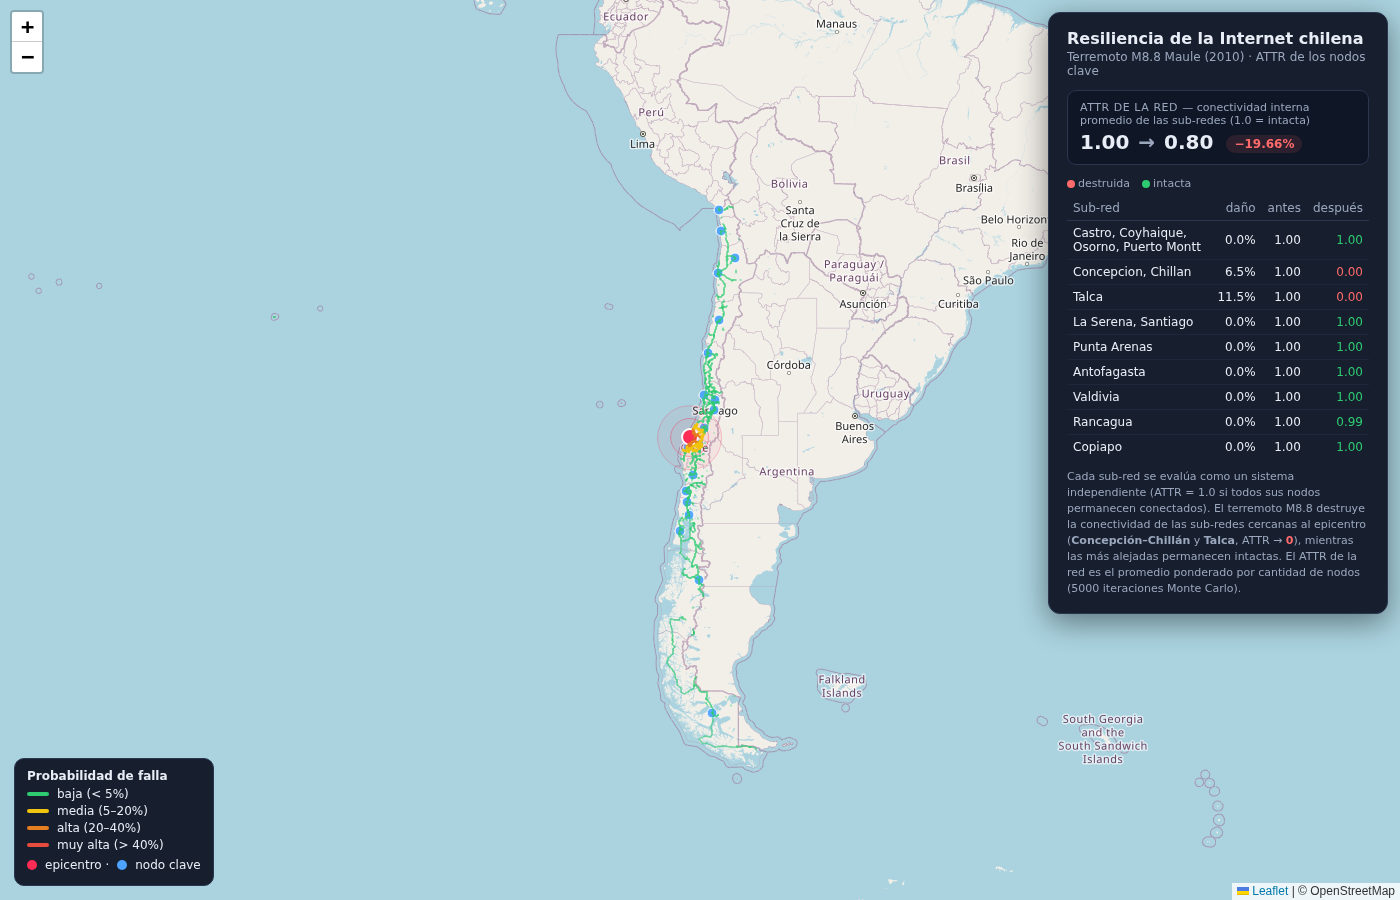
\includegraphics[width=\textwidth]{mapa_completo.png}
\caption{Mapa completo de la red de fibra chilena con daño sísmico y panel ATTR.
Los enlaces se colorean según su probabilidad de falla: verde (baja),
amarillo (media), naranja (alta), rojo (muy alta). El epicentro se marca
con anillos concéntricos.}
\label{fig:mapa}
\end{figure}

\begin{figure}[H]
\centering
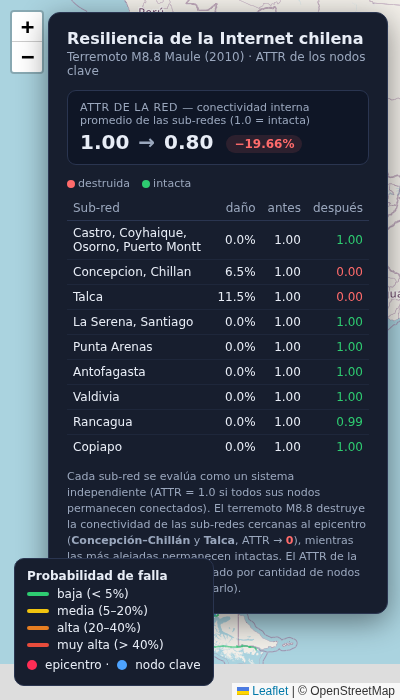
\includegraphics[width=0.45\textwidth]{panel_attr.png}
\caption{Panel lateral mostrando el ATTR de la red (1.00 $\to$ 0.80,
$-$19.66\%) y la tabla de ATTR por sub-red. Las sub-redes destruidas
(Concepción--Chillán y Talca) aparecen en rojo (ATTR = 0.00); las
intactas en verde.}
\label{fig:panel}
\end{figure}

El servidor expone tres APIs REST que alimentan el mapa: \texttt{/api/edges}
devuelve los enlaces operativos como GeoJSON con sus propiedades de falla,
\texttt{/api/nodos} los nodos clave, y \texttt{/api/attr} los resultados
del cálculo ATTR almacenados en la base de datos:

\begin{lstlisting}[language=Python,caption={APIs del servidor Flask (main.py)}]
@app.route("/api/edges")
def api_edges():
    return jsonify(q_geojson("""
        SELECT jsonb_build_object(
            'type','Feature',
            'geometry', ST_AsGeoJSON(geom)::jsonb,
            'properties', jsonb_build_object(
                'id', id, 'tipo', tipo,
                'p_fail', round(COALESCE(p_fail,0)::numeric,4),
                'dist_epi_km',
                  round(COALESCE(dist_epi_km,0)::numeric,1)))
        FROM edges WHERE operativo"""))

@app.route("/api/nodos")
def api_nodos():
    return jsonify(q_geojson("""
        SELECT jsonb_build_object(
            'type','Feature',
            'geometry', ST_AsGeoJSON(geom)::jsonb,
            'properties', jsonb_build_object(
                'cod',cod,'nombre',nombre,
                'rol',rol,'vertex_id',vertex_id))
        FROM nodos_clave"""))

@app.route("/api/attr")
def api_attr():
    r = leer_attr()
    return jsonify(r if r else {"error": "ejecute: python main.py attr"})
\end{lstlisting}


% ══════════════════════════════════════════════════════════════════
\section{Dockerización}

Para garantizar la reproducibilidad del proyecto, se construyó un entorno
Docker que ejecuta todo el \textit{pipeline} ---~desde la inicialización
de la base de datos hasta la visualización web~--- con un solo comando:

\begin{lstlisting}[language=bash,caption={Ejecución completa con Docker}]
docker compose up --build
\end{lstlisting}

La solución emplea un enfoque de \textbf{contenedor único} basado en la
imagen \texttt{postgres:17-bookworm}, sobre la cual se instalan PostGIS~3,
pgRouting y un entorno virtual Python con Flask.  Un script de entrada
(\texttt{docker-entrypoint.sh}) orquesta la secuencia completa: inicializa
el clúster PostgreSQL, construye la base de datos invocando
\texttt{main.py initdb}, calcula el ATTR mediante Monte Carlo
(\texttt{main.py attr -n 5000}) y finalmente levanta el servidor Flask
en \texttt{http://localhost:5000}.

\begin{lstlisting}[language=bash,caption={Secuencia del entrypoint (docker-entrypoint.sh)}]
# 1. Inicializar cluster PostgreSQL (si no existe)
su postgres -c "initdb -D $PGDATA"

# 2. Arrancar PostgreSQL
su postgres -c "pg_ctl -D $PGDATA start -w"

# 3. Construir BD y calcular ATTR (si la BD no existe)
python3 main.py initdb
python3 main.py attr -n 5000

# 4. Servir mapa web
exec python3 main.py serve --host 0.0.0.0 --port $PORT
\end{lstlisting}

Se utiliza \texttt{network\_mode: host} en \texttt{docker-compose.yml}
para que el contenedor comparta la pila de red del \textit{host},
evitando problemas de resolución DNS durante la construcción de la imagen.
La ejecución es \textbf{idempotente}: si la base de datos
\texttt{resiliencia} ya existe (por ejemplo, de una ejecución previa con
volúmenes persistentes), el contenedor omite la reconstrucción y levanta
directamente el servidor.

El puerto del servidor es configurable mediante la variable de entorno
\texttt{APP\_PORT} en \texttt{docker-compose.yml} (por defecto 5000).


% ══════════════════════════════════════════════════════════════════
\section{Estructura del repositorio}

\begin{lstlisting}[caption={Árbol de archivos del proyecto},language={}]
codigo-t2/
  main.py                 Orquestador (initdb / attr / serve / all)
  main.sql                Probabilidades de falla por enlace (entregable)
  requirements.txt        Dependencias Python
  Dockerfile              Imagen Docker (PG17+PostGIS+pgRouting+Flask)
  docker-compose.yml      Orquestacion Docker (un solo comando)
  docker-entrypoint.sh    Script de entrada del contenedor
  .dockerignore           Exclusiones para el build
  sql/
    00_pgr_createtopology_compat.sql  Compat. pgr_createTopology
    01_carga.sql          Extensiones PostGIS + pgRouting
    02_topologia.sql      Tabla edges + pgr_createTopology
    03_nodos_clave.sql    Nodos clave
    04_sismo.sql          Epicentro M8.8
    05_modelo_falla.sql   GMPE Campbell + fragilidad HAZUS
  scripts/
    attr.py               ATTR Monte Carlo
  templates/
    index.html            Mapa Leaflet
  data/
    shp/                  Shapefiles de infraestructura
    sismo_maule_2010.geojson
  docs/
    INFORME.tex           Este informe
    img/                  Capturas de pantalla
\end{lstlisting}


% ══════════════════════════════════════════════════════════════════
\section{Limitaciones}

El modelo presentado tiene limitaciones que conviene explicitar.  En
primer lugar, los identificadores de los shapefiles no son únicos ni
describen operador o capacidad, por lo que el modelo se apoya
exclusivamente en la geometría de los trazados.  En segundo lugar, la red
entregada por SUBTEL es una versión agregada (4~capas) de las 9 que
maneja el estudio original; parte de la fragmentación observada podría
deberse a huecos de digitalización y no necesariamente a desconexión
física real.  Finalmente, los parámetros $\mu$ y $\beta$ de la curva de
fragilidad, así como la GMPE de Campbell, son valores de primer orden
tomados de la literatura internacional.  Afinar estos parámetros con datos
específicos de la infraestructura de telecomunicaciones chilena ---~por
ejemplo, diferenciando entre fibra aérea, subterránea y submarina~---
mejoraría la calibración del modelo.  No obstante, todos los parámetros
son configurables en la tabla \texttt{modelo\_param}, lo que facilita la
experimentación con valores alternativos.


% ══════════════════════════════════════════════════════════════════
\begin{thebibliography}{99}

\bibitem{niclabs2018}
Universidad de Chile / NIC Labs (2018).
\emph{Estudio y Recomendaciones sobre la resiliencia de la infraestructura
de la Internet chilena}.
Informe Técnico Final CORFO 15BPE-47225.

\bibitem{boettcher2009}
N.\ Boettcher, Y.\ Prieto, S.E.\ Restrepo, J.E.\ Pezoa.
\emph{Resilient Multiculture Network Design in the Presence of
Exploit-Triggered Correlated Failures}.
IEEE/ACM Transactions on Networking.

\bibitem{campbell1981}
Campbell, K.W.\ (1981).
\emph{Near-source attenuation of peak horizontal acceleration}.
Bulletin of the Seismological Society of America, 71(6), 2039--2070.

\bibitem{hazus}
FEMA / NIBS.
\emph{HAZUS-MH Technical Manual}.
Capítulo sobre curvas de fragilidad lognormales para componentes de
comunicaciones y \textit{lifelines}.

\bibitem{valiant1979}
Valiant, L.G.\ (1979).
\emph{The complexity of enumeration and reliability problems}.
SIAM Journal on Computing, 8(3), 410--421.

\bibitem{ball1986}
Ball, M.O.\ (1986).
\emph{Computational complexity of network reliability analysis: An overview}.
IEEE Transactions on Reliability, R-35(3), 230--239.

\bibitem{fishman1986}
Fishman, G.S.\ (1986).
\emph{A Monte Carlo sampling plan for estimating network reliability}.
Operations Research, 34(4), 581--594.

\bibitem{gertsbakh2010}
Gertsbakh, I.B.\ y Shpungin, Y.\ (2010).
\emph{Models of Network Reliability: Analysis, Combinatorics, and Monte
Carlo}.
CRC Press.

\bibitem{eidinger2012}
Eidinger, J.M.\ y Tang, A.K.\ (2012).
\emph{Wastewater System Seismic Fragility Formulation}.
Journal of Infrastructure Systems, ASCE, 18(1).

\bibitem{abramowitz1964}
Abramowitz, M.\ y Stegun, I.A.\ (1964).
\emph{Handbook of Mathematical Functions with Formulas, Graphs, and
Mathematical Tables}.
National Bureau of Standards, Applied Mathematics Series~55.

\bibitem{usgs}
USGS Earthquake Catalog.
Evento \texttt{official20100227063411530\_30}.

\end{thebibliography}

\end{document}
